\documentclass{beamer}
\usepackage{../tut-slides}
\usepackage{../mathoperatorsAuD}

\usepackage[lighttt]{lmodern}
\usepackage{amsmath,amssymb}
\usepackage{stmaryrd}
\usepackage{enumerate}
%\usepackage[inline]{enumitem} 		%customize label
%\newcommand{\labelitemi}{\raisebox{1pt}{\scalebox{.9}{$\blacktriangleright$}}}
%\newcommand{\labelitemii}{$\vartriangleright$}
%\newcommand{\labelitemiii}{--}
\setbeamertemplate{itemize item}{\raisebox{1pt}{\scalebox{.9}{$\blacktriangleright$}}}
\setbeamertemplate{itemize subitem}{$\vartriangleright$}

\usepackage{booktabs}
\usepackage{tabularx}
\usepackage{tabu}
\newcommand*\head{\rowfont{\bfseries}}
\newcommand*{\tw}{\rowfont{\ttfamily}}
\renewcommand{\tabularxcolumn}[1]{>{\hspace{0pt}}m{#1}}
\usepackage{multirow}

\usepackage{cancel}

\usepackage{empheq}
\newcommand*\widefbox[1]{\fbox{\hspace{2em} #1 \hspace{2em}}}

\usepackage{tcolorbox}
\newtcolorbox{mymathbox}[1][]{colback=white, sharp corners, #1}

\usepackage{xcolor}
\usepackage{listings}
\lstset{numbers=left, 
	numberstyle=\tiny, 
	breaklines=true,
	backgroundcolor=\color{cdgray!20},
	numbersep=5pt,
	language=C,
	tabsize=2,
	basicstyle=\footnotesize\ttfamily,
	showstringspaces=false} 

\DeclareMathOperator{\ack}{\mathbf{ack}}
\usepackage{MnSymbol}

\newcommand{\col}[1]{\textcolor{cdpurple}{#1}}
\newcolumntype{R}[1]{>{\centering\arraybackslash}p{#1}}

\begin{document}	
	\title{Algorithmen und Datenstrukturen}
	\subtitle{Übung 7: Pulsierender Speicher \& Listen}
	\author{Eric Kunze}
	\email{eric.kunze@mailbox.tu-dresden.de}
	\city{TU Dresden}
%	\institute{Lehrstuhl für Grundlagen der Programmierung}
	\titlegraphic{
\includegraphics[width=2cm]{../TUD-white.pdf}}
	\date{05.12.2019}

	\maketitle


%%%%%%%%%%%%%%%%%%%%%%%%%%%%%%%%%%%%%%%%%%%%%%%%%%%%%%%%%%%%%%%%%%%%%%%%%%%%%
\begin{frame} \frametitle{Aufgabe 1}
	\centering
	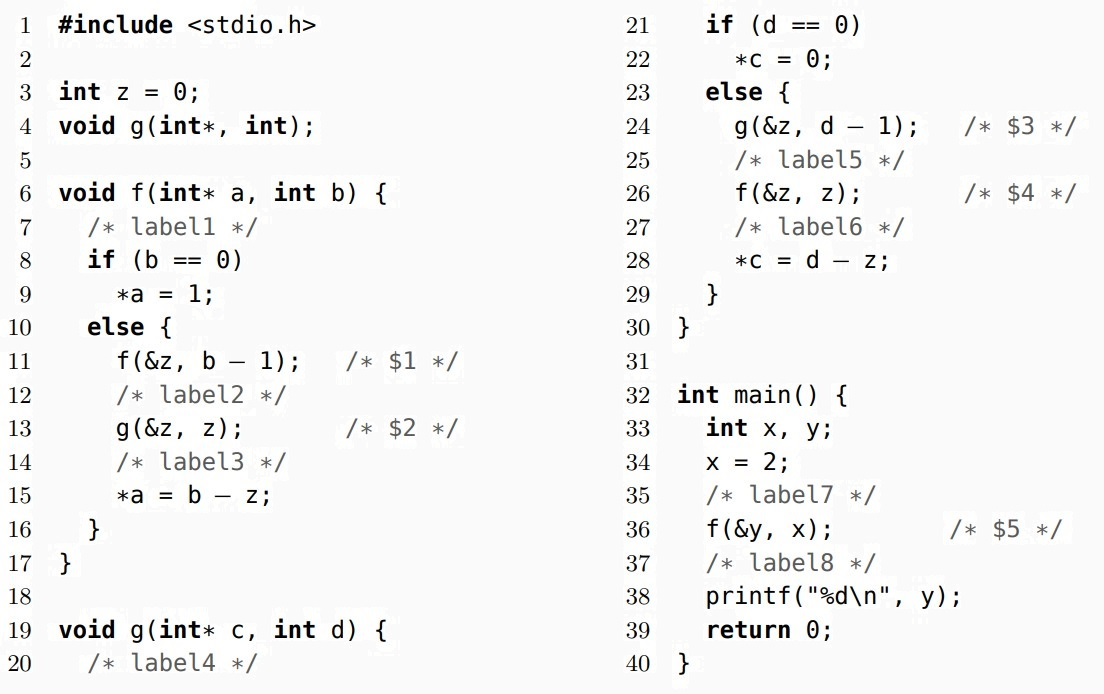
\includegraphics[width=\textwidth]{./tut07_aufgabe1.jpg}
\end{frame}

\begin{frame} \frametitle{Aufgabe 1 --- Teil (a)}
	\textbf{Gültigkeitsbereiche}
	
	\centering
	\begin{tabular}{|l|c|}
		\hline
		Objektname & Gültigkeitsbereich \\ \hline \hline
		\texttt{z} & 3 -- 40 \\ \hline
		\texttt{g} & 4 -- 40 \\ \hline
		\texttt{f} & 6 -- 40 \\ \hline
		\texttt{a,b} in \texttt{f} & 6 -- 17 \\ \hline
		\texttt{c,d} in \texttt{g} & 19 -- 30 \\ \hline
		\texttt{main} & 32 -- 40 \\ \hline
		\texttt{x,y} in \texttt{main} & 33 -- 40 \\ \hline
	\end{tabular}
\end{frame}

\begin{frame} \frametitle{Aufgabe 1 --- Teil (b)}
		\centering
		\def\arraystretch{0.9}
	
		\begin{tabular}{|p{1.4cm}|r||R{0.3cm}|R{0.3cm}|R{0.3cm}|R{0.3cm}|R{0.3cm}|R{0.3cm}|R{0.3cm}|R{0.3cm}|R{0.3cm}|R{0.3cm}|}
			\hline
			Label & RM & 1 & 2 & 3 & 4 & 5 & 6 & 7 & 8 & 9 & 10 \\ 
			\hline \hline
			\multirow{2}[0]{*}{\texttt{label7}} & \multirow{2}[0]{*}{--} & z & x & y &       &       &       &       &       &  &\\
			&       & 0     & 2     & ? &       &       &       &       &       &  &\\ \hline
			\multirow{2}[0]{*}{\texttt{label1}} & \multirow{2}[0]{*}{5} & z &       &       & a & b &       &       &       &  &\\
			&       & 0     &       &       & 3     & 2     &       &       &       & & \\ \hline
			\multirow{2}[0]{*}{\texttt{label1}} & \multirow{2}[0]{*}{1:5} & z &       &       &       &       & a & b &       &  &\\
			&       & 0     &       &       &       &       & 1     & 1     &       &  &\\ \hline
			\multirow{2}[0]{*}{\texttt{label1}} & \multirow{2}[0]{*}{1:1:5} & z &       &       &       &       &       &       & a & b &\\
			&       & 0     &       &       &       &       &       &       & 1     & 0 &\\ \hline
			\multirow{2}[0]{*}{\texttt{label2}} & \multirow{2}[0]{*}{1:5} & z &       &       &       &       & a & b &       & & \\
			&       & 0     &       &       &       &       & 1     & 1     &       &  & \\ \hline
		\end{tabular}
\end{frame}

\begin{frame} \frametitle{Aufgabe 1 --- Teil (b)}
	\centering
	\small
	\def\arraystretch{0.9}
	
	\begin{tabular}{|p{1.4cm}|r||R{0.2cm}|R{0.2cm}|R{0.2cm}|R{0.2cm}|R{0.2cm}|R{0.2cm}|R{0.2cm}|R{0.2cm}|R{0.2cm}|R{0.2cm}|R{0.2cm}|}
		\hline
		Label & RM & 1 & 2 & 3 & 4 & 5 & 6 & 7 & 8 & 9 & 10 & 11 \\ 
		\hline \hline
		\multirow{2}[0]{*}{\texttt{label4}} & \multirow{2}[0]{*}{2:1:5} & z &  &  &       &       &       &       & c & d & &\\
		&       & 1     & 2     & ? & 3     & 2     & 1     & 1     & 1     & 1  &&\\ \hline
		\multirow{2}[0]{*}{\texttt{label4}} & \multirow{2}[0]{*}{3:2:1:5} & z &       &       &  &  &       &       &       &  & c & d\\
		&       & 1    &       &       &      &      &       &       &       & & 1 & 0 \\ \hline
		\multirow{2}[0]{*}{\texttt{label5}} & \multirow{2}[0]{*}{2:1:5} & z &       &       &       &       &  &  &      c & d & &\\
		&       & 0     &       &       &       &       &      &      &  1     & 1 & &\\ \hline
		\multirow{2}[0]{*}{\texttt{label1}} & \multirow{2}[0]{*}{4:2:1:5} & z &       &       &       &       &       &       & & & a & b\\
		&       & 0     &       &       &       &       &       &       &      &  & 1 & 0\\ \hline
		\multirow{2}[0]{*}{\texttt{label6}} & \multirow{2}[0]{*}{2:1:5} & z &       &       &       &       &  &  &      c & d& & \\
		&       & 1     &       &       &       &       &      &      &  1  & 1 & & \\ \hline
	\end{tabular}
\end{frame}

\begin{frame} \frametitle{Aufgabe 1 --- Teil (b)}
	\centering
	\def\arraystretch{0.9}
	
	\begin{tabular}{|p{1.4cm}|r||R{0.3cm}|R{0.3cm}|R{0.3cm}|R{0.3cm}|R{0.3cm}|R{0.3cm}|R{0.3cm}|R{0.3cm}|R{0.3cm}|R{0.3cm}|}
		\hline
		Label & RM & 1 & 2 & 3 & 4 & 5 & 6 & 7 & 8 & 9 & 10 \\ 
		\hline \hline
		\multirow{2}[0]{*}{\texttt{label5}} & \multirow{2}[0]{*}{2:5} & z &  &  &       &       & c      & d      &       &  &\\
		&       & 0     & 2     & ? & 3     & 2     & 1     & 1     &       &  &\\ \hline
		\multirow{2}[0]{*}{\texttt{label1}} & \multirow{2}[0]{*}{4:2:5} & z &       &       &  &  &       &       &      a & b &\\
		&       & 0     &       &       &      &    &       &       &      1 & 0 & \\ \hline
		\multirow{2}[0]{*}{\texttt{label6}} & \multirow{2}[0]{*}{2:5} & z &       &       &       &       & c & d &       &  &\\
		&       & 1     &       &       &       &       & 1     & 1     &       &  &\\ \hline
		\multirow{2}[0]{*}{\texttt{label3}} & \multirow{2}[0]{*}{5} & z &        &       & a     & b     &       &       &  &  &\\
		&       & 0     &       &       & 3     & 2     &       &       &      &  &\\ \hline
		\multirow{2}[0]{*}{\texttt{label8}} & \multirow{2}[0]{*}{--} & z &  x    & y     &      &       &  &  &       & & \\
		&       & 0     & 2     & 2     &       &       &     &     &       &  & \\ \hline
	\end{tabular}
\end{frame}


%%%%%%%%%%%%%%%%%%%%%%%%%%%%%%%%%%%%%%%%%%%%%%%%%%%%%%%%%%%%%%%%%%%%%%%%%%%%%%%%%%%


%%%%%%%%%%%%%%%%%%%%%%%%%%%%%%%%%%%%%%%%%%%%%%%%%%%%%%%%%%%%%%%%%%%%%%%%%%%%%%%%%%%





%%%%%%%%%%%%%%%%%%%%%%%%%%%%%%%%%%%%%%%%%%%%%%%%%%%%%%%%%%%%%%%%%%%%%%%%%%%%%%%%%%%

\end{document}